\section{Graetz-Gleichrichter}
\subsection{Experimentelle Durchf\"uhrung}
Als erstes wird die Greatz-Gleichrichter Schaltung aus Abbildung 8 auf dem Steckbrett und im PSpice nachgebaut. Es Werden vier Dioden (Typ: \textbf{1N4148}), ein Widerstand R$_1$ $=$ 1~$k\Omega$ und drei unterschiedliche Kapazit\"aten verwendet. Zun\"achst wird die Brummspannung d\"ur alle Varianten(mit und ohne Kapzit\"at) bestimmt. Anschlie\ss end wird eine konstante Kapazit\"at(C$_1$ $=$ 1~$\mu F$) angeschlossen und die Brummspannung wird unter variablen Widerst\"aden bestimmt. 
\begin{figure}[!h]
\begin{center}
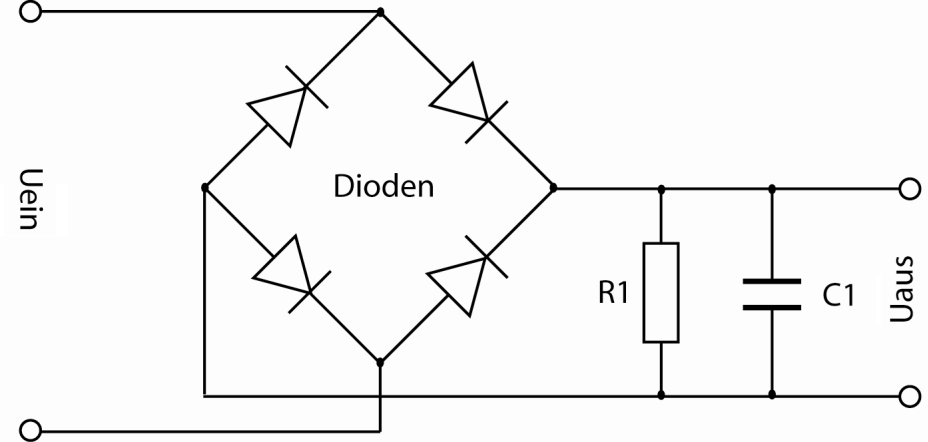
\includegraphics[scale=0.4]{schaltungVersuch3}
\caption{Greatz-Gleichrichter}
\end{center}
\end{figure}
\newpage
\subsection{Ergebnisse und Diskussion}
\begin{figure}[!h]
\begin{minipage}{0.5\textwidth}
\begin{center}
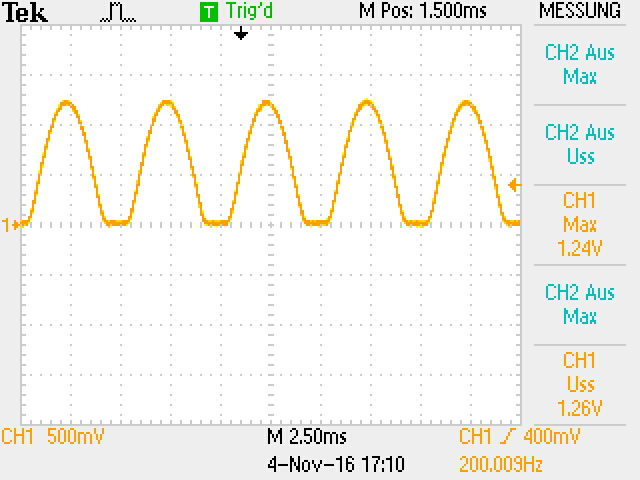
\includegraphics[scale=0.6]{bilder/Versuch2/ohnekondensator}
\caption{Greatz-Gleichrichter ohne Kondensator}
\end{center}
\end{minipage}
\hfill
\begin{minipage}{0.4\textwidth}
\begin{center}
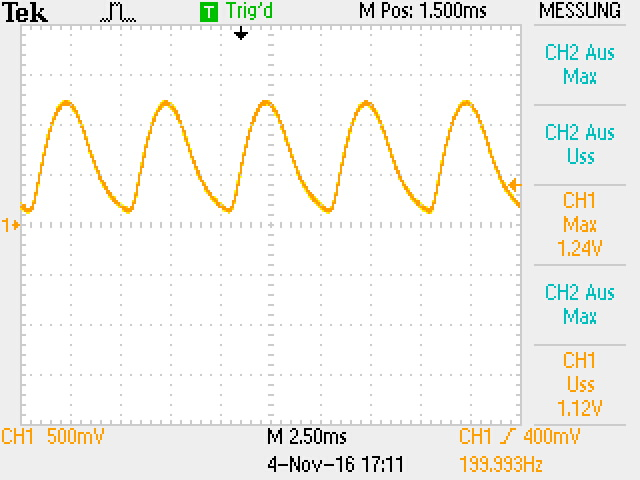
\includegraphics[scale=0.6]{bilder/Versuch2/mitkondensator}
\caption{Greatz-Gleichrichter mit C$_1$ $=$1~$\mu F$}
\end{center}
\end{minipage}

\end{figure}

\begin{figure}[!h]
\begin{minipage}{0.4\textwidth}
\begin{center}
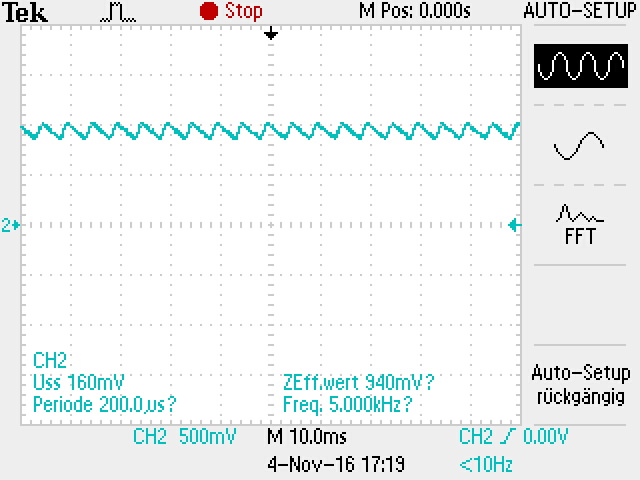
\includegraphics[scale=0.6]{bild/TEK0002}
\caption{Greatz-Gleichrichter mit C$_1$ $=$ 22~$\mu F$}
\end{center}
\end{minipage}
\hfill
\begin{minipage}{0.4\textwidth}
\begin{center}
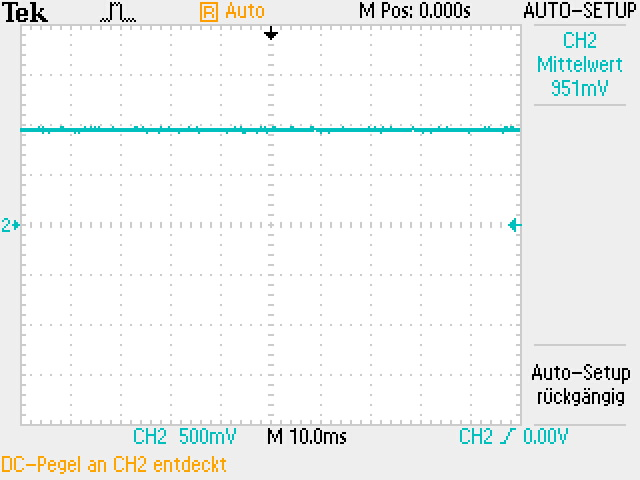
\includegraphics[scale=0.6]{bild/TEK0003}
\caption{Greatz-Gleichrichter mit C$_1$ $=$ 470~$\mu F$}
\end{center}
\end{minipage}

\end{figure}
\newpage
\begin{table}[!h]
\begin{center}
\caption{Messergebnisse Brummspannung}
\begin{tabular}{|l|l|l|l}
\hline
C/$\mu F$ & Brummspannung/$mV$ \\
\hline
0 & 1200\\
\hline
1 & 1000 \\
\hline
22 & 160 \\
\hline
470 & $\approx$ 0\\
\hline
\end{tabular}
\end{center}
\end{table}
\noindent
Die Brummspannung wird mit steigender Kapazit\"at geringer und schlie\ss lich geht sie gegen null. Der Grund Daf\"ur ist, dass die Spannung am Ausgang sich mit gr\"o\ss er Kapazit\"aten immer st\"arker gl\"atet.


\begin{figure}[!h]
\begin{center}
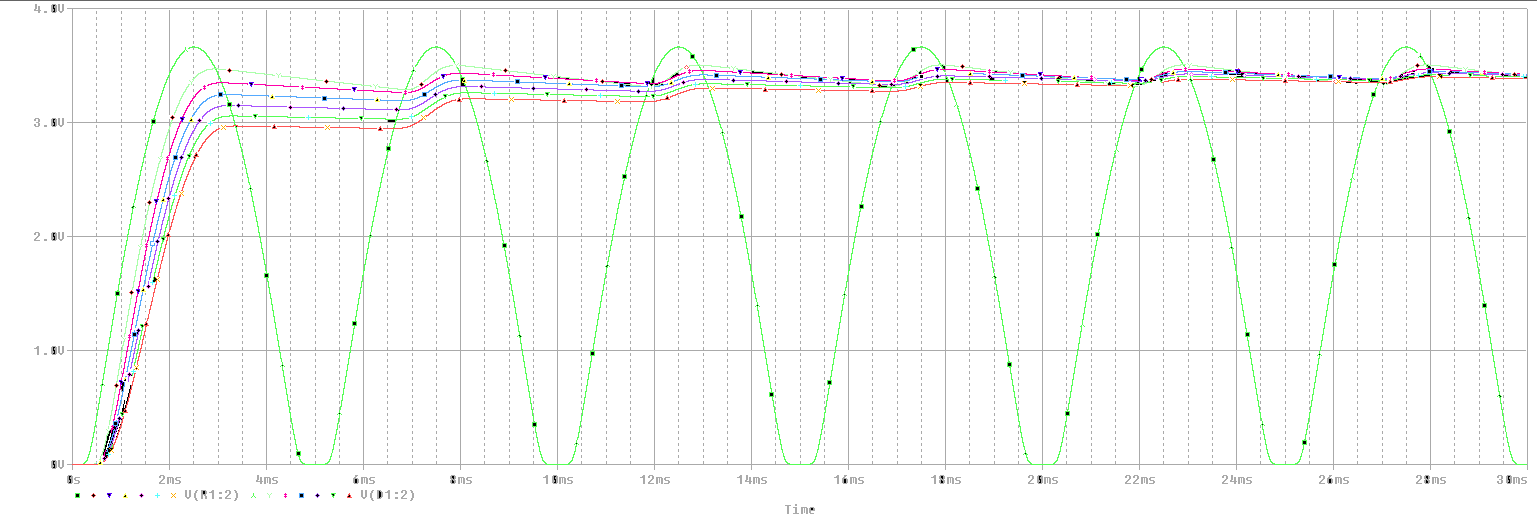
\includegraphics[width=0.8\textwidth]{Versuch3-SimulationmitVariablenKondesator}
\caption{Simulationsergebnisse Greatz-Gleichrichter mit unterschiedlichen Kapazit\"aten}
\end{center}
\end{figure}
Ein Vergleich zu den Simulierten Ergebnissen bringt ein \"ahnliches Bild. Die Brummspannung sinkt mit steigender Kapazit\"at, da die Ausgangsspannung immer st\"arker gegl\"attet wird. 
\newpage
\begin{figure}
\begin{minipage}{0.4\textwidth}
\begin{center}
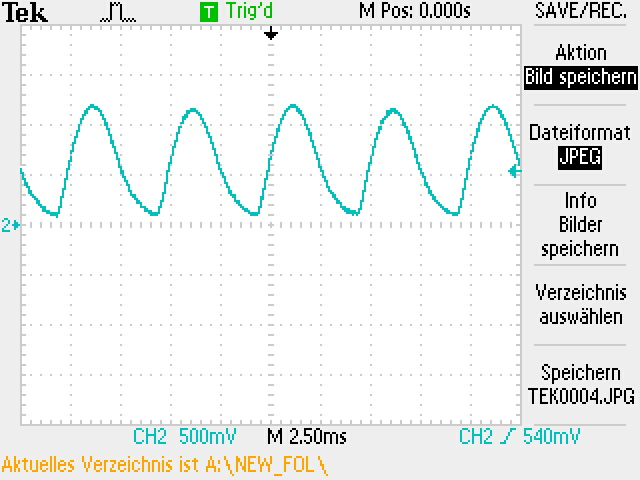
\includegraphics[scale=0.7]{bild/TEK0004}
\caption{Greatz-Gleichrichter mit R$_1$ $=$ 1~$k\Omega$}
\end{center}
\end{minipage}
\hfill
\begin{minipage}{0.4\textwidth}
\begin{center}
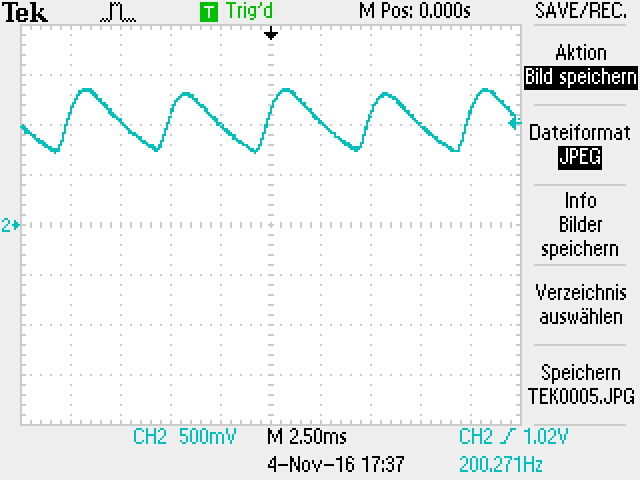
\includegraphics[scale=0.7]{bild/TEK0005}
\caption{Greatz-Gleichrichter  mit R$_1$ $=$ 6~$k\Omega$}
\end{center}
\end{minipage}
\end{figure}
\begin{figure}
\begin{center}
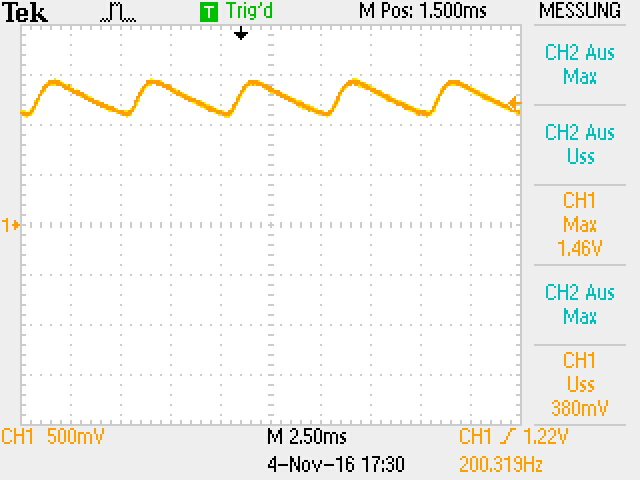
\includegraphics[scale=0.7]{bilder/Versuch2/12widerstand}
\caption{Greatz-Gleichrichter mit R$_1$ $=$ 12 $K \Omega$}
\end{center}
\end{figure}
\begin{table}[!h]
\begin{center}
\caption{Messwerte Brummspannung}
\begin{tabular}{|l|l|}\hline
R$_1$/$k\Omega$ & Brummspannung/$V$ \\
\hline
1 & 1.1 \\
\hline
6 & 0.6 \\
\hline
12 & 0.3 \\
\hline

\end{tabular}
\end{center}
\end{table}
\noindent
Es zeigt sich, dass mit steigenden Widerstandswerten die Brummspannung geringer wird. Dies ist der Fall, weil an dem Widerstand R$_1$ mehr Spannung abf\"allt, sodass sich der Kondensator schneller entleert. 
\subsubsection{Greatz-Gleichrichter Variante 2: Widerst\"ande}
\begin{figure}[ht]
\begin{center}
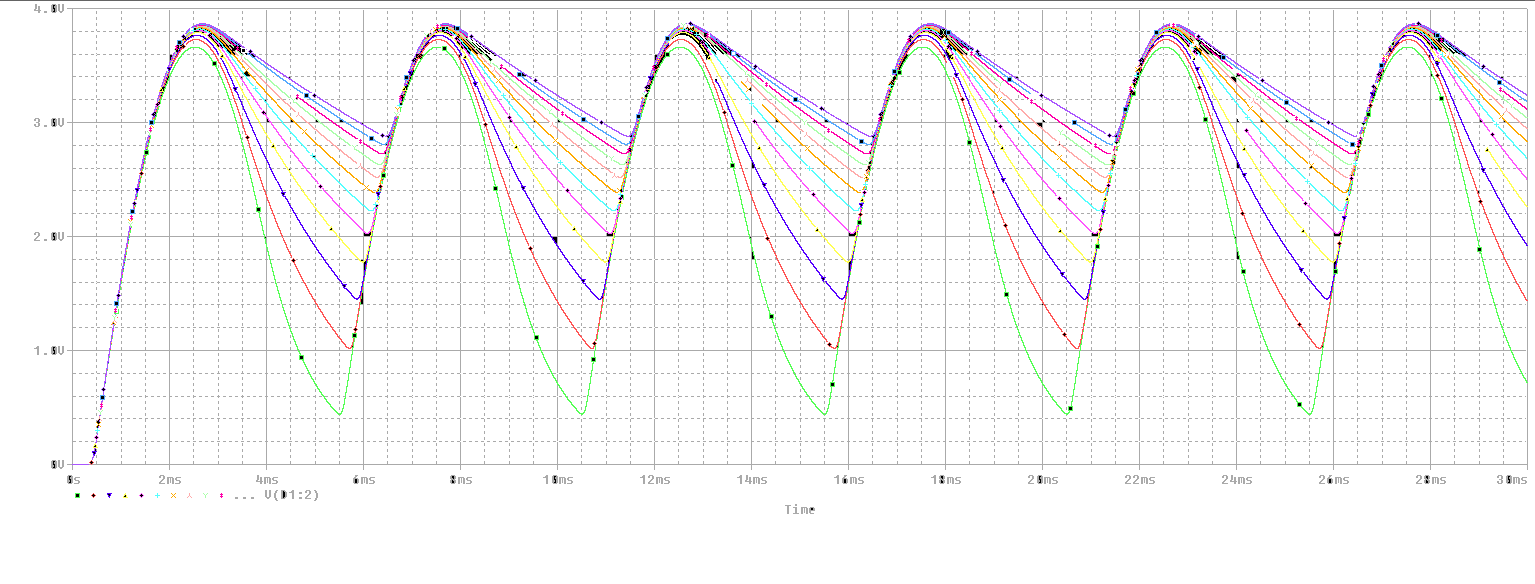
\includegraphics[width=0.8\textwidth]{Versuch3-SimulationmitVariablenWiderstand}
\caption{Simulationsergebnisse Greatz-Gleichrichter mit unterschiedlichen Widerst\"anden}
\end{center}
\end{figure}
\noindent
Ein Vergleich zu dem simulierten Ergebnissen zeigt wiederum ein \"ahnliches Bild mit steigenden Widerst\"anden wird die Brummspannung geringer. 